\documentclass{standalone}
\usepackage{pgf,tikz,pgfplots}
\pgfplotsset{compat=1.15}
\usepackage{mathrsfs}
\pagestyle{empty}
\begin{document}
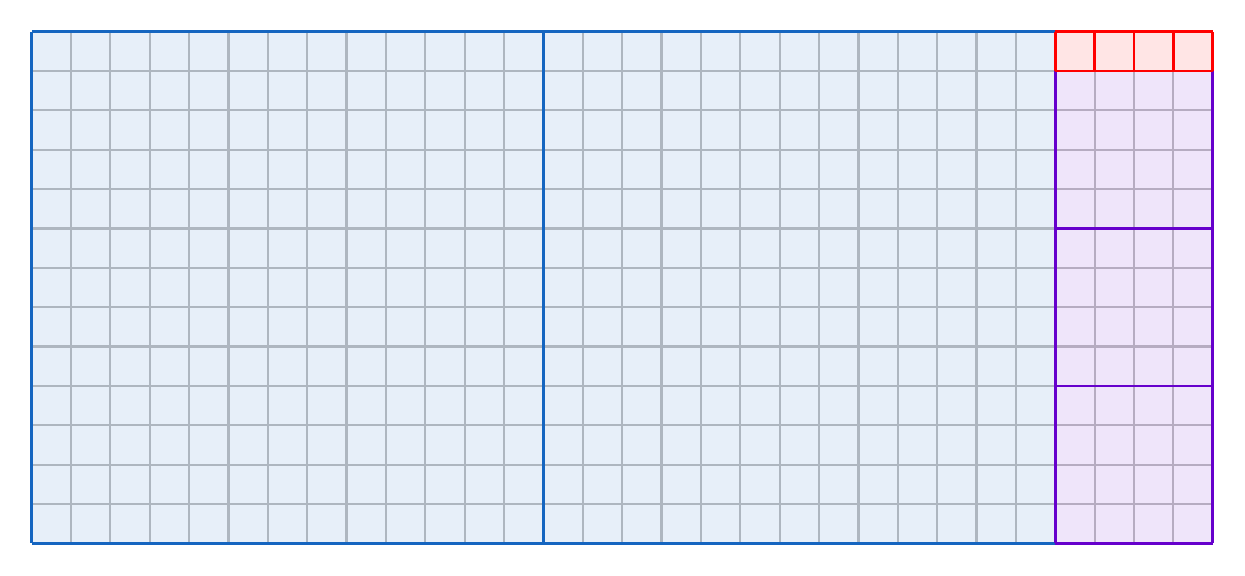
\begin{tikzpicture}[thick,scale=0.5]
\definecolor{ffqqqq}{rgb}{1,0,0}
\definecolor{wwqqcc}{rgb}{0.4,0,0.8}
\definecolor{rvwvcq}{rgb}{0.08235294117647059,0.396078431372549,0.7529411764705882}
\definecolor{cqcqcq}{rgb}{0.7529411764705882,0.7529411764705882,0.7529411764705882}
\draw [color=cqcqcq,, xstep=1cm,ystep=1cm] (0,0) grid (30,13);
\clip(-0.1,-0.1) rectangle (30.1,13.1);
\fill[line width=1pt,color=rvwvcq,fill=rvwvcq,fill opacity=0.10000000149011612] (0,13) -- (0,0) -- (13,0) -- (13,13) -- cycle;
\fill[line width=1pt,color=rvwvcq,fill=rvwvcq,fill opacity=0.10000000149011612] (13,13) -- (13,0) -- (26,0) -- (26,13) -- cycle;
\fill[line width=1pt,color=wwqqcc,fill=wwqqcc,fill opacity=0.1] (26,0) -- (30,0) -- (30,4) -- (26,4) -- cycle;
\fill[line width=1pt,color=wwqqcc,fill=wwqqcc,fill opacity=0.1] (26,4) -- (30,4) -- (30,8) -- (26,8) -- cycle;
\fill[line width=1pt,color=wwqqcc,fill=wwqqcc,fill opacity=0.1] (26,8) -- (30,8) -- (30,12) -- (26,12) -- cycle;
\fill[line width=1pt,color=ffqqqq,fill=ffqqqq,fill opacity=0.10000000149011612] (26,13) -- (26,12) -- (27,12) -- (27,13) -- cycle;
\fill[line width=1pt,color=ffqqqq,fill=ffqqqq,fill opacity=0.1] (27,13) -- (27,12) -- (28,12) -- (28,13) -- cycle;
\fill[line width=1pt,color=ffqqqq,fill=ffqqqq,fill opacity=0.1] (28,13) -- (28,12) -- (29,12) -- (29,13) -- cycle;
\fill[line width=1pt,color=ffqqqq,fill=ffqqqq,fill opacity=0.1] (29,13) -- (29,12) -- (30,12) -- (30,13) -- cycle;
\draw [line width=1pt,color=rvwvcq] (0,13)-- (0,0);
\draw [line width=1pt,color=rvwvcq] (0,0)-- (13,0);
\draw [line width=1pt,color=rvwvcq] (13,0)-- (13,13);
\draw [line width=1pt,color=rvwvcq] (13,13)-- (0,13);
\draw [line width=1pt,color=rvwvcq] (13,13)-- (13,0);
\draw [line width=1pt,color=rvwvcq] (13,0)-- (26,0);
\draw [line width=1pt,color=rvwvcq] (26,0)-- (26,13);
\draw [line width=1pt,color=rvwvcq] (26,13)-- (13,13);
\draw [line width=1pt,color=wwqqcc] (26,0)-- (30,0);
\draw [line width=1pt,color=wwqqcc] (30,0)-- (30,4);
\draw [line width=1pt,color=wwqqcc] (30,4)-- (26,4);
\draw [line width=1pt,color=wwqqcc] (26,4)-- (26,0);
\draw [line width=1pt,color=wwqqcc] (26,4)-- (30,4);
\draw [line width=1pt,color=wwqqcc] (30,4)-- (30,8);
\draw [line width=1pt,color=wwqqcc] (30,8)-- (26,8);
\draw [line width=1pt,color=wwqqcc] (26,8)-- (26,4);
\draw [line width=1pt,color=wwqqcc] (26,8)-- (30,8);
\draw [line width=1pt,color=wwqqcc] (30,8)-- (30,12);
\draw [line width=1pt,color=wwqqcc] (30,12)-- (26,12);
\draw [line width=1pt,color=wwqqcc] (26,12)-- (26,8);
\draw [line width=1pt,color=ffqqqq] (26,13)-- (26,12);
\draw [line width=1pt,color=ffqqqq] (26,12)-- (27,12);
\draw [line width=1pt,color=ffqqqq] (27,12)-- (27,13);
\draw [line width=1pt,color=ffqqqq] (27,13)-- (26,13);
\draw [line width=1pt,color=ffqqqq] (27,13)-- (27,12);
\draw [line width=1pt,color=ffqqqq] (27,12)-- (28,12);
\draw [line width=1pt,color=ffqqqq] (28,12)-- (28,13);
\draw [line width=1pt,color=ffqqqq] (28,13)-- (27,13);
\draw [line width=1pt,color=ffqqqq] (28,13)-- (28,12);
\draw [line width=1pt,color=ffqqqq] (28,12)-- (29,12);
\draw [line width=1pt,color=ffqqqq] (29,12)-- (29,13);
\draw [line width=1pt,color=ffqqqq] (29,13)-- (28,13);
\draw [line width=1pt,color=ffqqqq] (29,13)-- (29,12);
\draw [line width=1pt,color=ffqqqq] (29,12)-- (30,12);
\draw [line width=1pt,color=ffqqqq] (30,12)-- (30,13);
\draw [line width=1pt,color=ffqqqq] (30,13)-- (29,13);
\end{tikzpicture}
\end{document}